% FoodBridge — End-Semester Project Report
% UCS503P Software Engineering Laboratory, Group 3
% Structure follows the course report template.
\documentclass[11pt,a4paper]{report}

\usepackage[margin=1in]{geometry}
\usepackage[T1]{fontenc}
\usepackage{lmodern}
\usepackage{graphicx}
\usepackage{booktabs}
\usepackage{array}
\usepackage{tabularx}
\usepackage{enumitem}
\usepackage{xcolor}
\usepackage{float}
\usepackage{caption}
\usepackage{subcaption}
\usepackage{tikz}
\usetikzlibrary{arrows.meta,positioning,shapes.geometric}
\usepackage[hidelinks]{hyperref}
\usepackage{titlesec}
\usepackage{fancyhdr}
\usepackage{pdflscape}

\definecolor{fbgreen}{HTML}{1F6F52}
\titleformat{\chapter}[display]{\normalfont\Large\bfseries\color{fbgreen}}{Chapter \thechapter}{8pt}{\LARGE}
\titlespacing*{\chapter}{0pt}{0pt}{20pt}
\titleformat{\section}{\large\bfseries}{\thesection}{0.6em}{}
\titleformat{\subsection}{\normalsize\bfseries}{\thesubsection}{0.6em}{}

\pagestyle{fancy}
\fancyhf{}
\fancyhead[L]{\small FoodBridge --- End-Semester Report}
\fancyhead[R]{\small Group 3}
\fancyfoot[C]{\small\thepage}
\renewcommand{\headrulewidth}{0.4pt}
\fancypagestyle{plain}{\fancyhf{}\fancyfoot[C]{\small\thepage}\renewcommand{\headrulewidth}{0pt}}

\newcommand{\code}[1]{\texttt{\detokenize{#1}}}
\setlist{itemsep=2pt,topsep=4pt}
\captionsetup{font=small,labelfont=bf}
\setlength{\parskip}{4pt}

\begin{document}

% ------------------------------------------------------------------ title
\begin{titlepage}
\centering
{\large UCS503P - Software Engineering Laboratory\par}
\vspace{3cm}
{\Huge\bfseries FoodBridge\par}
\vspace{0.5cm}
{\Large A Surplus Food Redistribution Matcher\par}
\vspace{3cm}
\begin{tabular}{ll}
1024030119 & Hardik Pajiala \\
1024030916 & Shikhar Goel \\
1024030164 & Ayush Shukla \\
\end{tabular}
\par\vspace{1.2cm}
{\large Group: 3 \quad BE Third Year, Computer Engineering\par}
\vspace{0.4cm}
{\large Advisor: Ms.\ Anushka\par}
\vfill
{\large End-Semester Evaluation\par}
\vspace{0.8cm}
{\large Computer Science and Engineering Department\par}
{\large Thapar Institute of Engineering and Technology, Patiala\par}
\end{titlepage}

\tableofcontents
\clearpage

% ============================================================ Chapter 1
\chapter{Introduction}

\section{Background and Context}

Restaurants, hostel messes, caterers and event organisers routinely end the day
with cooked food they cannot sell or serve. At the same time, shelters, NGOs,
orphanages and community kitchens within a few kilometres of them often have
people they cannot feed. The two are rarely connected. When they are, it is
usually through a phone call or a message to someone who happens to know
someone, which works only if the right person answers before the food spoils.

Cooked food has a window of a few hours. That makes the problem one of
\emph{matching under a deadline} rather than one of logistics in general: the
food has to reach an organisation that is close enough to collect it in time,
that has the capacity to use it, and that can actually accept that kind of food.
Getting any one of those wrong means the food is wasted anyway, only later and
further away.

FoodBridge is a web application that makes that match explicitly. A donor posts
surplus food and its pickup address; an administrator approves the listing; and
a matching engine offers it to the single organisation best placed to use it,
recording why it chose that organisation over every other one it considered.

\subsection{Problem Statement}

Informal redistribution has three weaknesses this project addresses directly.

\begin{itemize}
  \item \textbf{No eligibility check.} A broadcast message reaches organisations
    that are too far away, already full, or unable to accept the food type. The
    donor has no way to know which recipients are realistic.
  \item \textbf{No record of decisions.} When food goes to one organisation and
    not another, nothing records why. An unfair or inefficient pattern cannot be
    noticed, let alone corrected.
  \item \textbf{No handling of failure.} If nobody responds, the food is simply
    lost. There is no queue, no retry, and no measurement of how often it happens.
\end{itemize}

\section{Project Objectives}

The objectives were fixed in the project proposal and carried unchanged into
the Software Requirements Specification.

\begin{enumerate}
  \item \textbf{Allocate on explicit criteria.} Every offer is made by an
    algorithm whose inputs and weights are written down and configurable, not
    by whoever replies first.
  \item \textbf{Make every allocation explainable.} For each donation the system
    stores, and shows, every organisation it considered, whether it was eligible,
    and the reason it was excluded if it was not.
  \item \textbf{Never silently drop food.} A donation with no eligible recipient
    is widened in search radius and then waitlisted for retry, not discarded.
  \item \textbf{Measure the outcome.} Time-to-match, rescue rate, first-offer
    acceptance and distance travelled are computed from stored timestamps, so the
    project can be judged on what it delivered rather than on its design.
\end{enumerate}

% ============================================================ Chapter 2
\chapter{Methodology and Design}

\section{System Architecture}

\subsection{High-Level Design}

FoodBridge is split into three services around one spatial database
(Figure~\ref{fig:arch}). The split is deliberate: allocation is the part of the
system most likely to change, so it lives behind its own HTTP boundary, where
the strategy can be replaced without touching the API or the interface.

\begin{figure}[H]
\centering
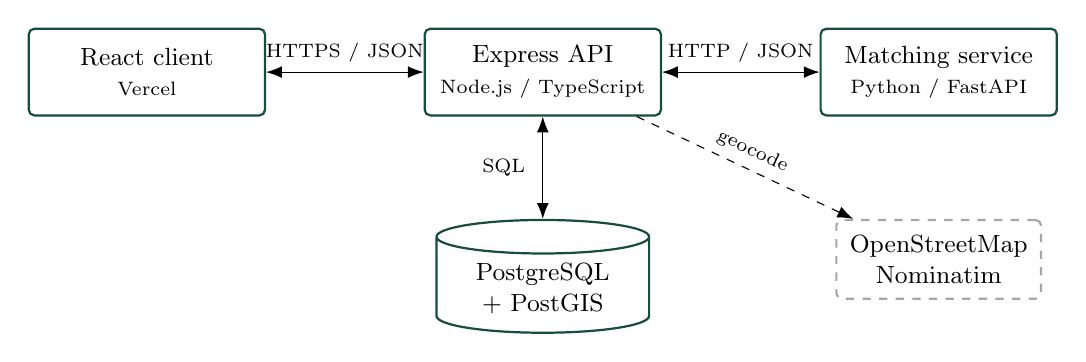
\begin{tikzpicture}[
  box/.style={draw=fbgreen!70!black, thick, rounded corners=2pt, align=center,
              minimum width=30mm, minimum height=11mm, font=\small},
  ext/.style={draw=gray!70, thick, dashed, rounded corners=2pt, align=center,
              minimum width=26mm, minimum height=10mm, font=\small},
  store/.style={draw=fbgreen!70!black, thick, cylinder, shape border rotate=90,
                aspect=0.22, align=center, minimum width=27mm,
                minimum height=13mm, font=\small},
  lbl/.style={font=\scriptsize, midway, sloped, above}
]
\node[box] (web) {React client\\\scriptsize Vercel};
\node[box, right=20mm of web] (api) {Express API\\\scriptsize Node.js / TypeScript};
\node[box, right=20mm of api] (match) {Matching service\\\scriptsize Python / FastAPI};
\node[store, below=13mm of api] (db) {PostgreSQL\\+ PostGIS};
\node[ext, below=13mm of match] (nom) {OpenStreetMap\\Nominatim};

\draw[{Latex[length=2mm]}-{Latex[length=2mm]}] (web) -- node[lbl]{HTTPS / JSON} (api);
\draw[{Latex[length=2mm]}-{Latex[length=2mm]}] (api) -- node[lbl]{HTTP / JSON} (match);
\draw[{Latex[length=2mm]}-{Latex[length=2mm]}] (api) -- node[font=\scriptsize,left=1mm]{SQL} (db);
\draw[-{Latex[length=2mm]}, dashed] (api) -- node[font=\scriptsize,sloped,above]{geocode} (nom);
\end{tikzpicture}
\caption{High-level architecture. Addresses are resolved through Nominatim and
cached in PostgreSQL; distances and radius searches run in PostGIS.}
\label{fig:arch}
\end{figure}

A request follows one path regardless of who makes it. The React client calls
the Express API; the API authenticates the caller, enforces the state machine,
and reads or writes the database. Only a matching cycle reaches the matching
service: the API gathers every open donation, uses PostGIS to compute the
distance from each donation to every organisation within the maximum radius,
and sends the result to the matcher, which returns assignments together with a
per-candidate explanation.

\subsection{Technical Stack}

\begin{table}[H]
\centering
\small
\begin{tabularx}{\linewidth}{@{}l>{\raggedright\arraybackslash}X@{}}
\toprule
\textbf{Layer} & \textbf{Technology and reason} \\
\midrule
Interface & React 18 with Vite. Role-aware routing so donors, organisations and
  administrators each see only their own screens. \\
API & Express with TypeScript. Every status change goes through one central
  state machine, so an illegal transition is refused in one place. \\
Matching & Python and FastAPI, with SciPy for the Hungarian assignment
  (\code{linear_sum_assignment}). \\
Database & PostgreSQL 17 with PostGIS 3.6. Locations are
  \code{GEOGRAPHY(Point,4326)} with GiST indexes, so distances are real
  great-circle distances rather than arithmetic on latitude and longitude. \\
Geocoding & OpenStreetMap Nominatim, behind a database cache. \\
Authentication & JSON Web Tokens, passwords hashed with bcrypt. \\
Testing & Vitest and Supertest for the API against a real PostGIS database;
  pytest for the matcher; a contract checker for the client--server boundary. \\
CI and hosting & GitHub Actions runs every suite on each push; the client is
  hosted on Vercel. \\
\bottomrule
\end{tabularx}
\caption{Technical stack.}
\end{table}

\subsection{System Modelling and UML Diagrams}

The diagrams in this section were drawn from the implemented code, not from the
proposal. The state machine in particular is taken transition for transition
from the API's own state-machine module, \code{stateMachines.ts}, which is what
every status change is checked against.

\paragraph{Use Case Diagram.}
Figure~\ref{fig:usecase} shows three human actors --- donor, recipient
organisation and administrator --- and two system actors, the geocoding service
and the notification service, together with the include and extend
relationships between use cases.

\begin{landscape}
\begin{figure}[p]
\centering
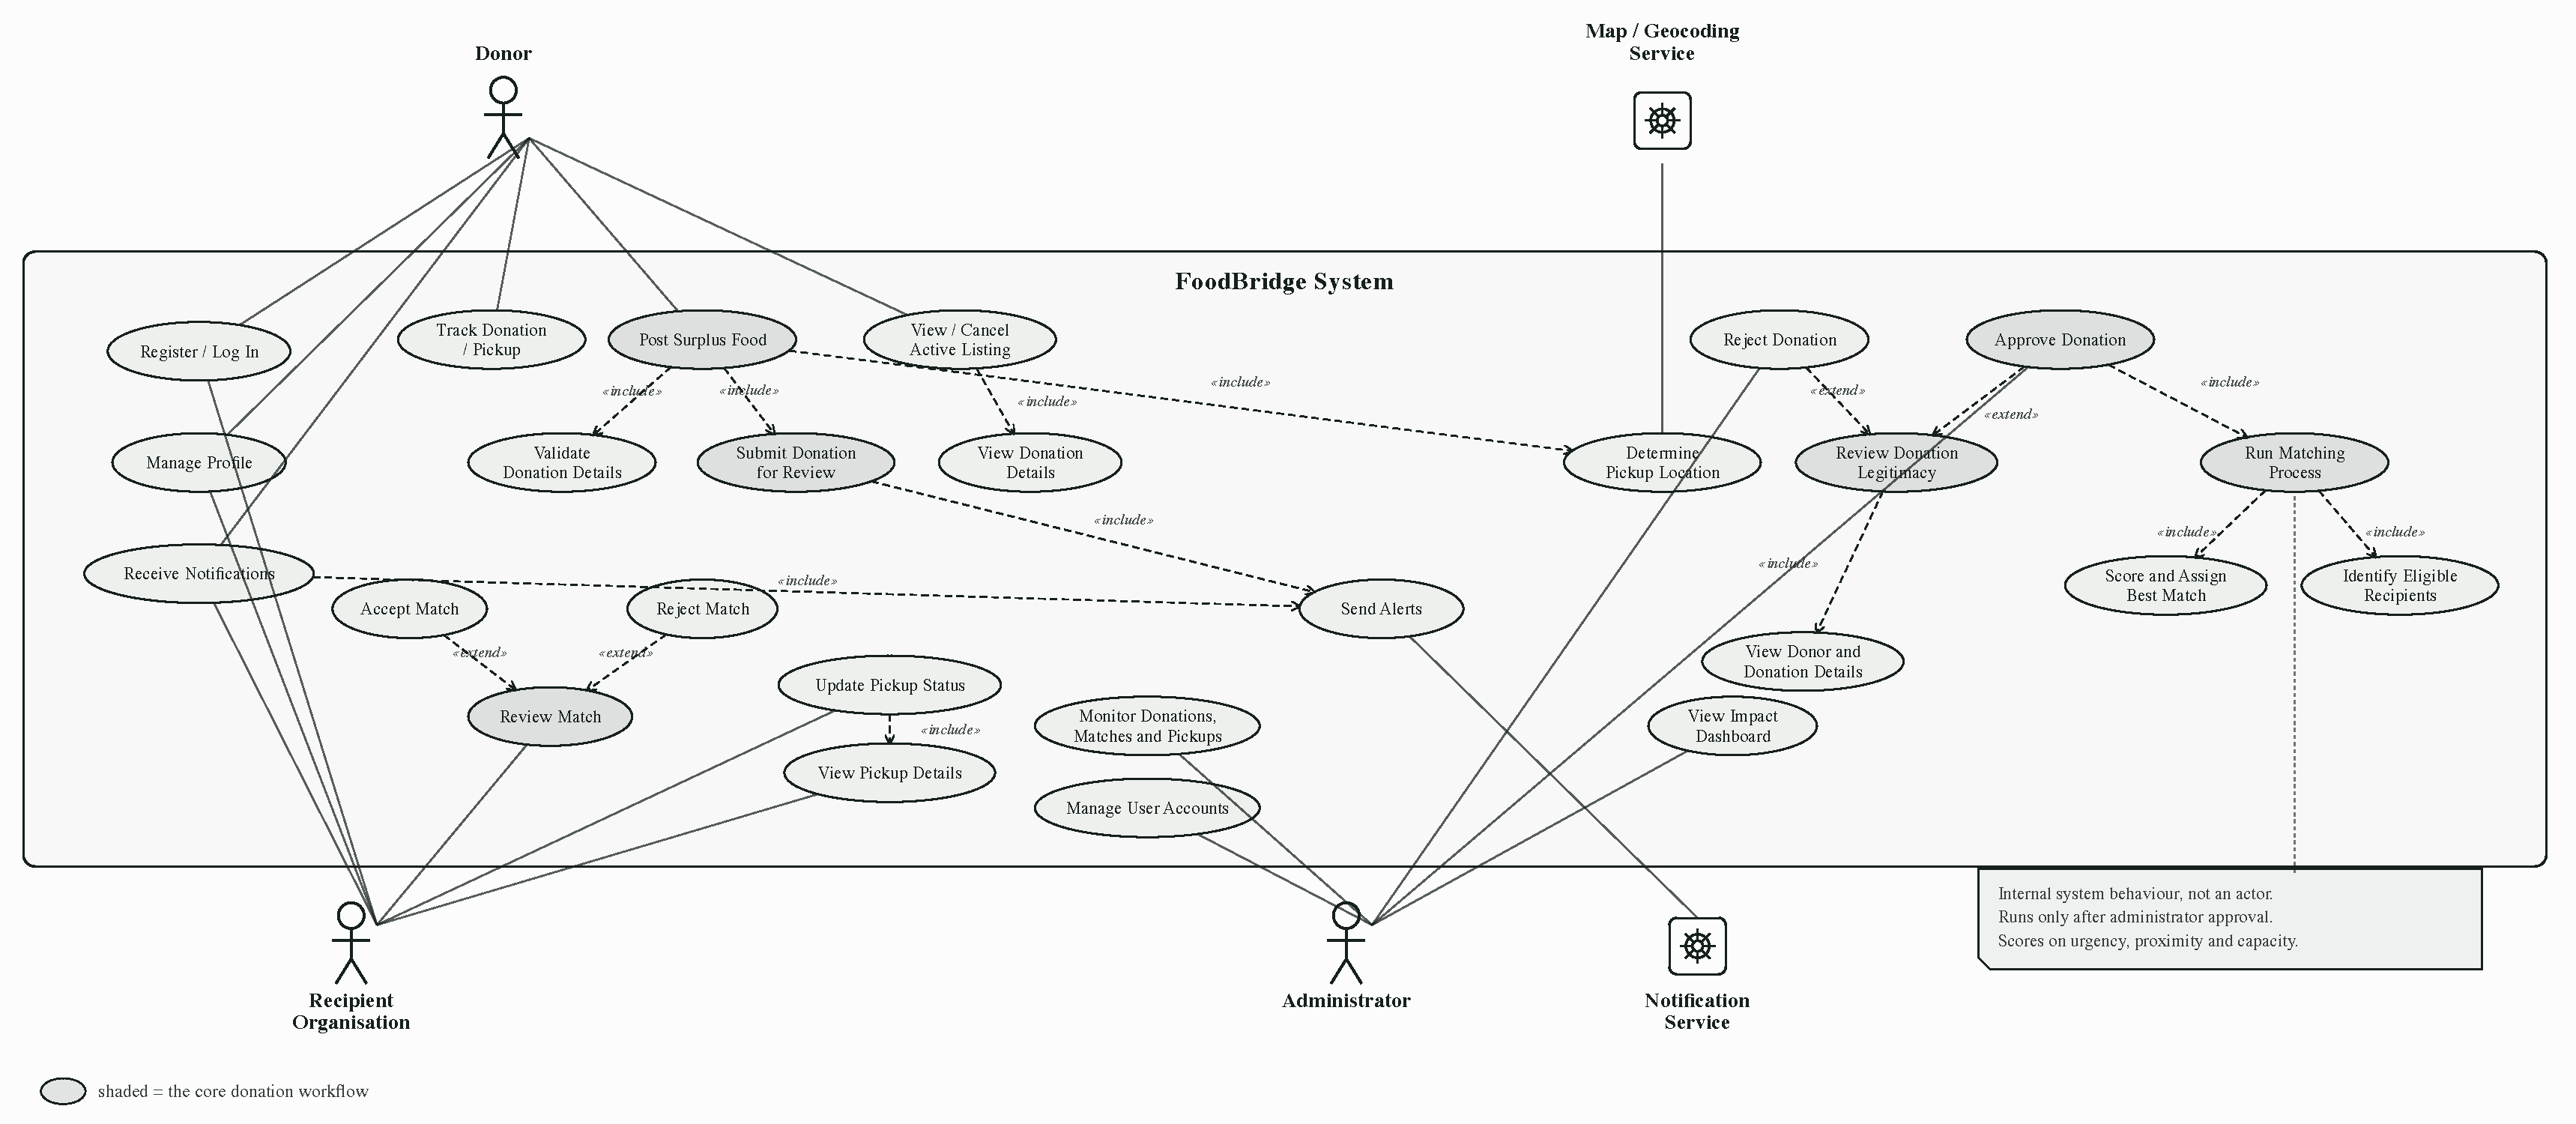
\includegraphics[width=\linewidth]{figures/use-case.pdf}
\caption{Use case diagram. Dashed arrows are \emph{include} (behaviour the base
use case always performs) and \emph{extend} (behaviour that occurs only under a
condition).}
\label{fig:usecase}
\end{figure}
\end{landscape}

\paragraph{Class Diagram.}
Figure~\ref{fig:class} shows the fourteen persistent entities. Donors and
recipient organisations specialise a common user. A donation is offered as
zero or more matches, and an accepted match becomes a pickup. Three entities
exist purely to make decisions inspectable: \code{MatchingRun} and
\code{MatchExplanation} record what every cycle considered, and
\code{StatusEvent} is the audit trail of who changed what and when. The
geocoding cache has no foreign key; it is a dependency of the two entities whose
locations it resolves.

\begin{figure}[H]
\centering
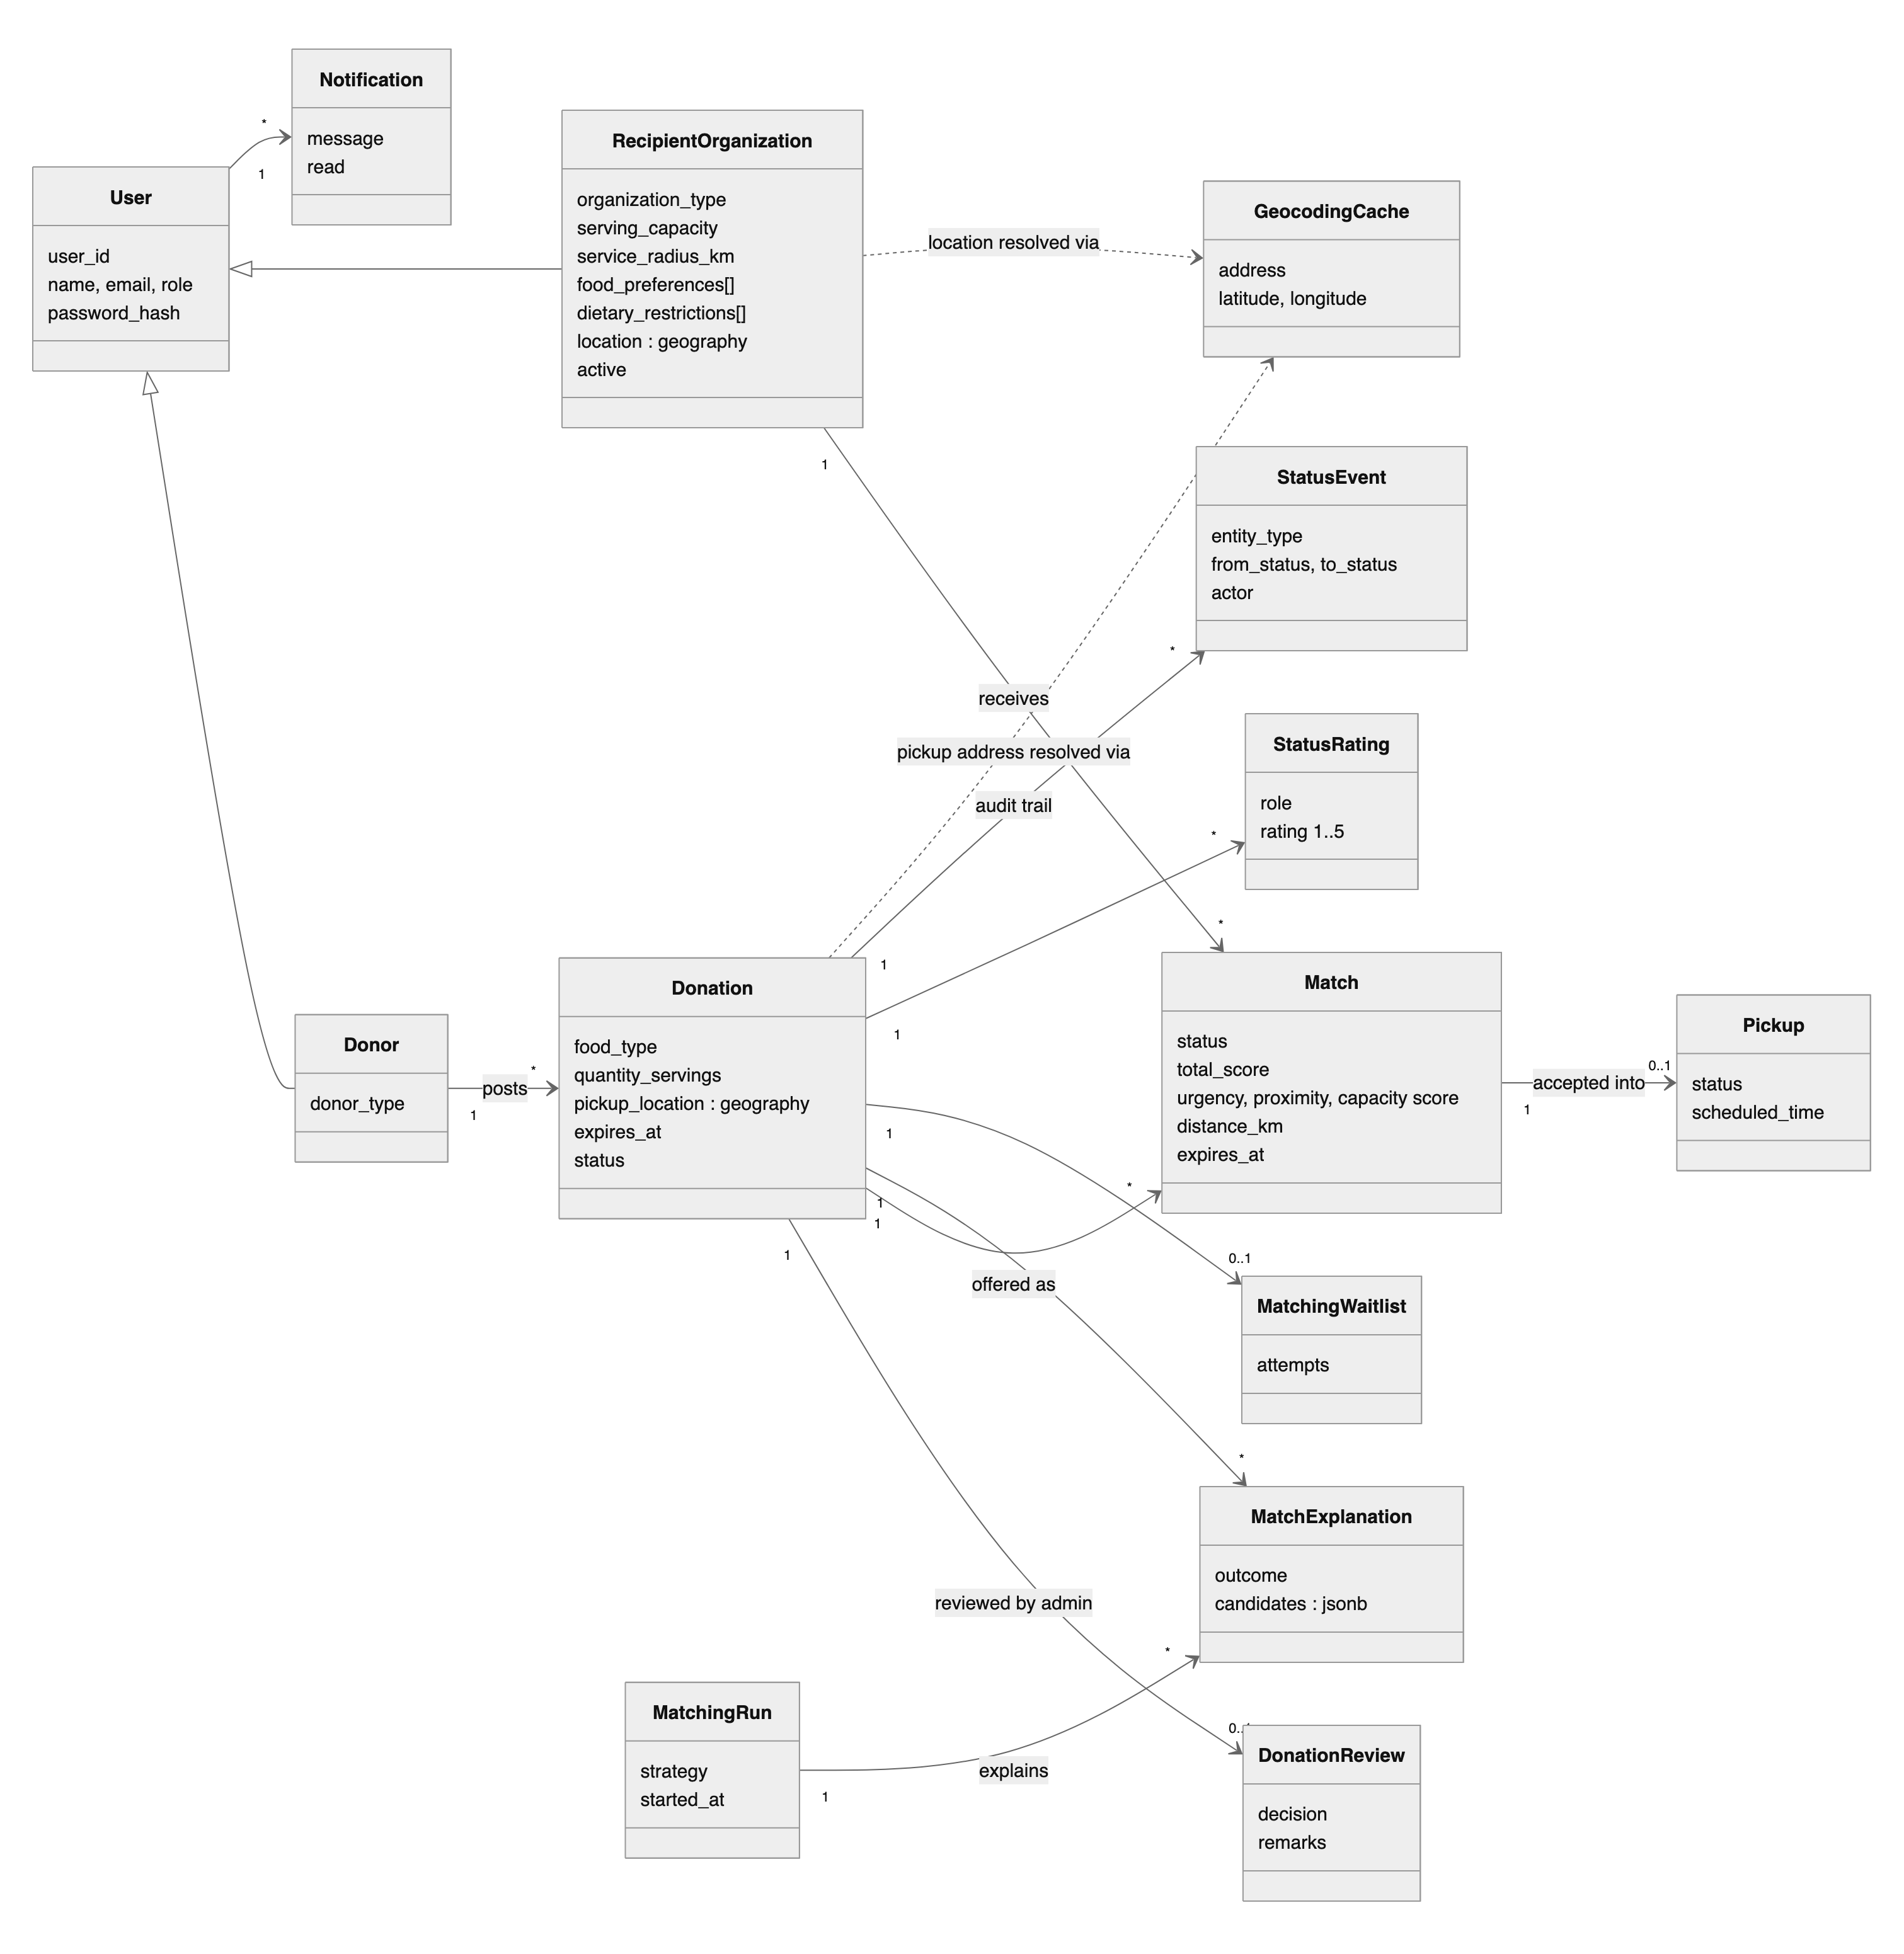
\includegraphics[width=\linewidth]{figures/class.png}
\caption{Class diagram of the persistent model.}
\label{fig:class}
\end{figure}

\paragraph{State Machine Diagram.}
A donation's lifecycle is the most important rule in the system, and the one
most worth getting exactly right (Figure~\ref{fig:state}). A new donation waits
for an administrator before anyone can see it. The \code{MATCHED} to
\code{POSTED} transition is the re-match loop: when an offer is declined or not
answered within thirty minutes, the donation returns to the pool rather than
being lost. Any non-terminal state can expire once the food's deadline passes,
and that expiry runs unattended every sixty seconds.

\begin{figure}[H]
\centering
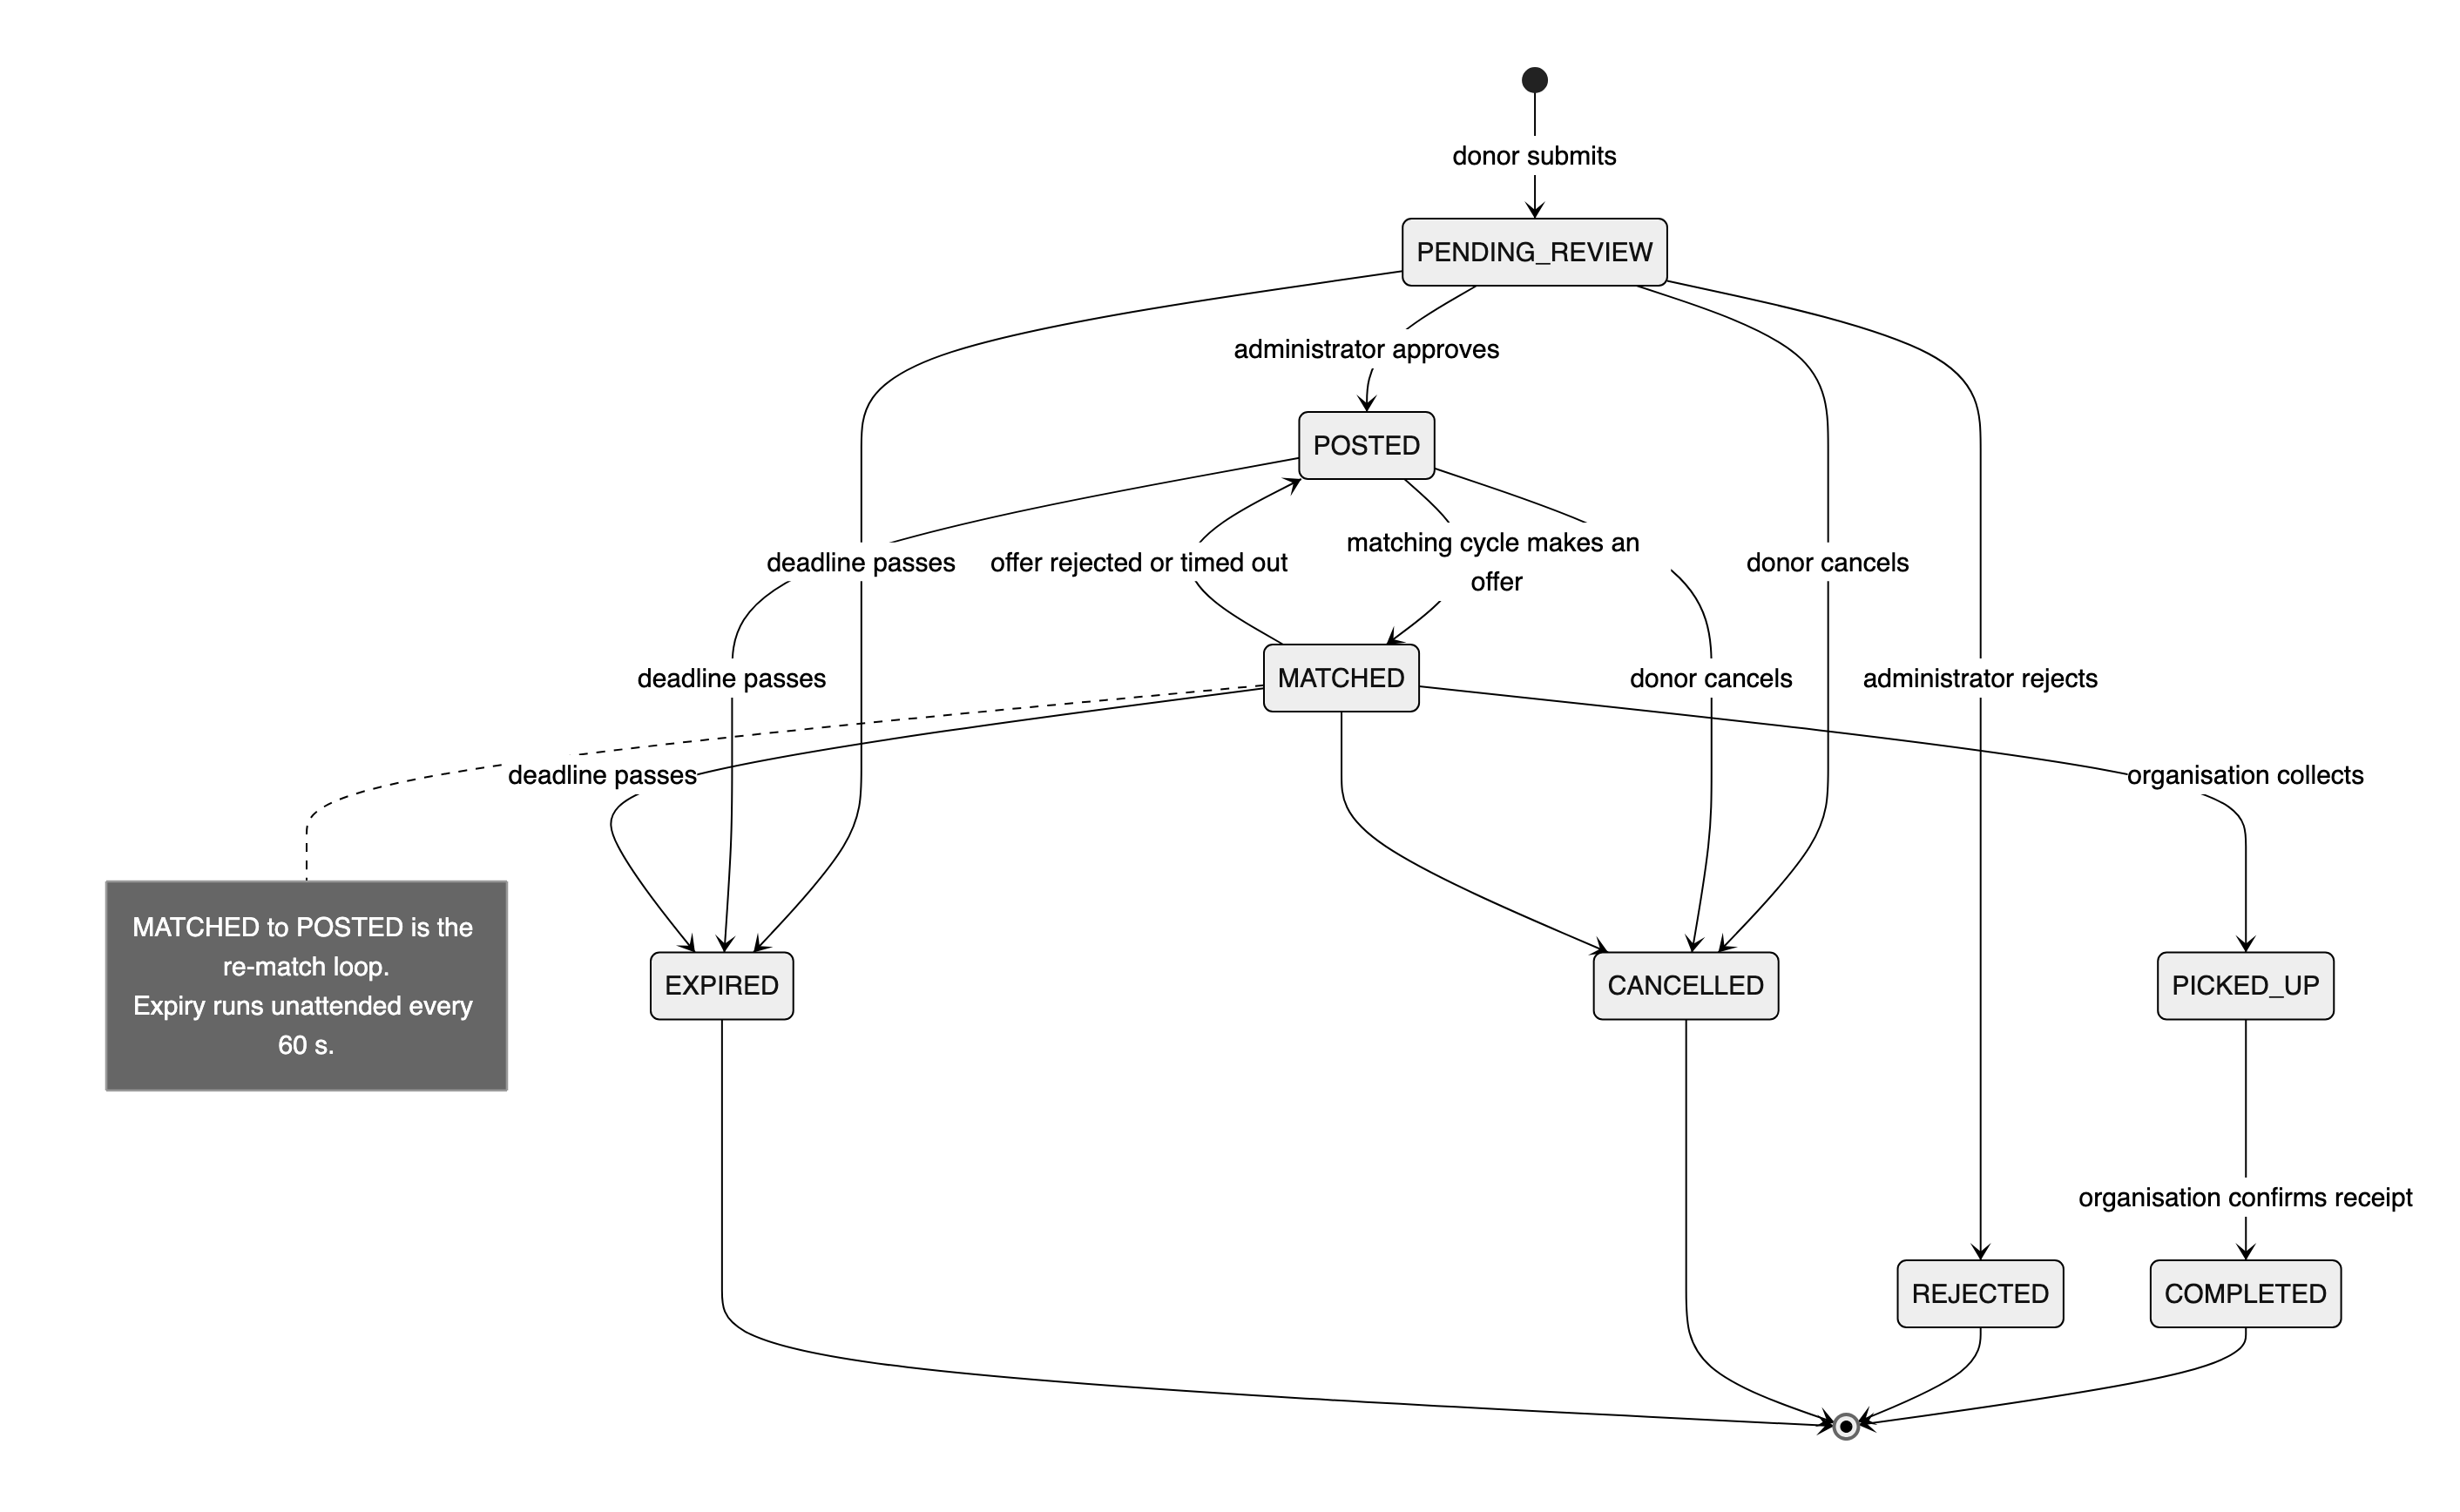
\includegraphics[width=\linewidth]{figures/state.png}
\caption{Donation state machine, as enforced by the API.}
\label{fig:state}
\end{figure}

\paragraph{Activity Diagram.}
Figure~\ref{fig:activity} shows a matching cycle. Its defining property is that
eligibility is decided \emph{before} any scoring. An organisation that fails one
of seven hard filters never competes on score at all, which is why the nearest
organisation is frequently not the one that wins.

\begin{figure}[H]
\centering
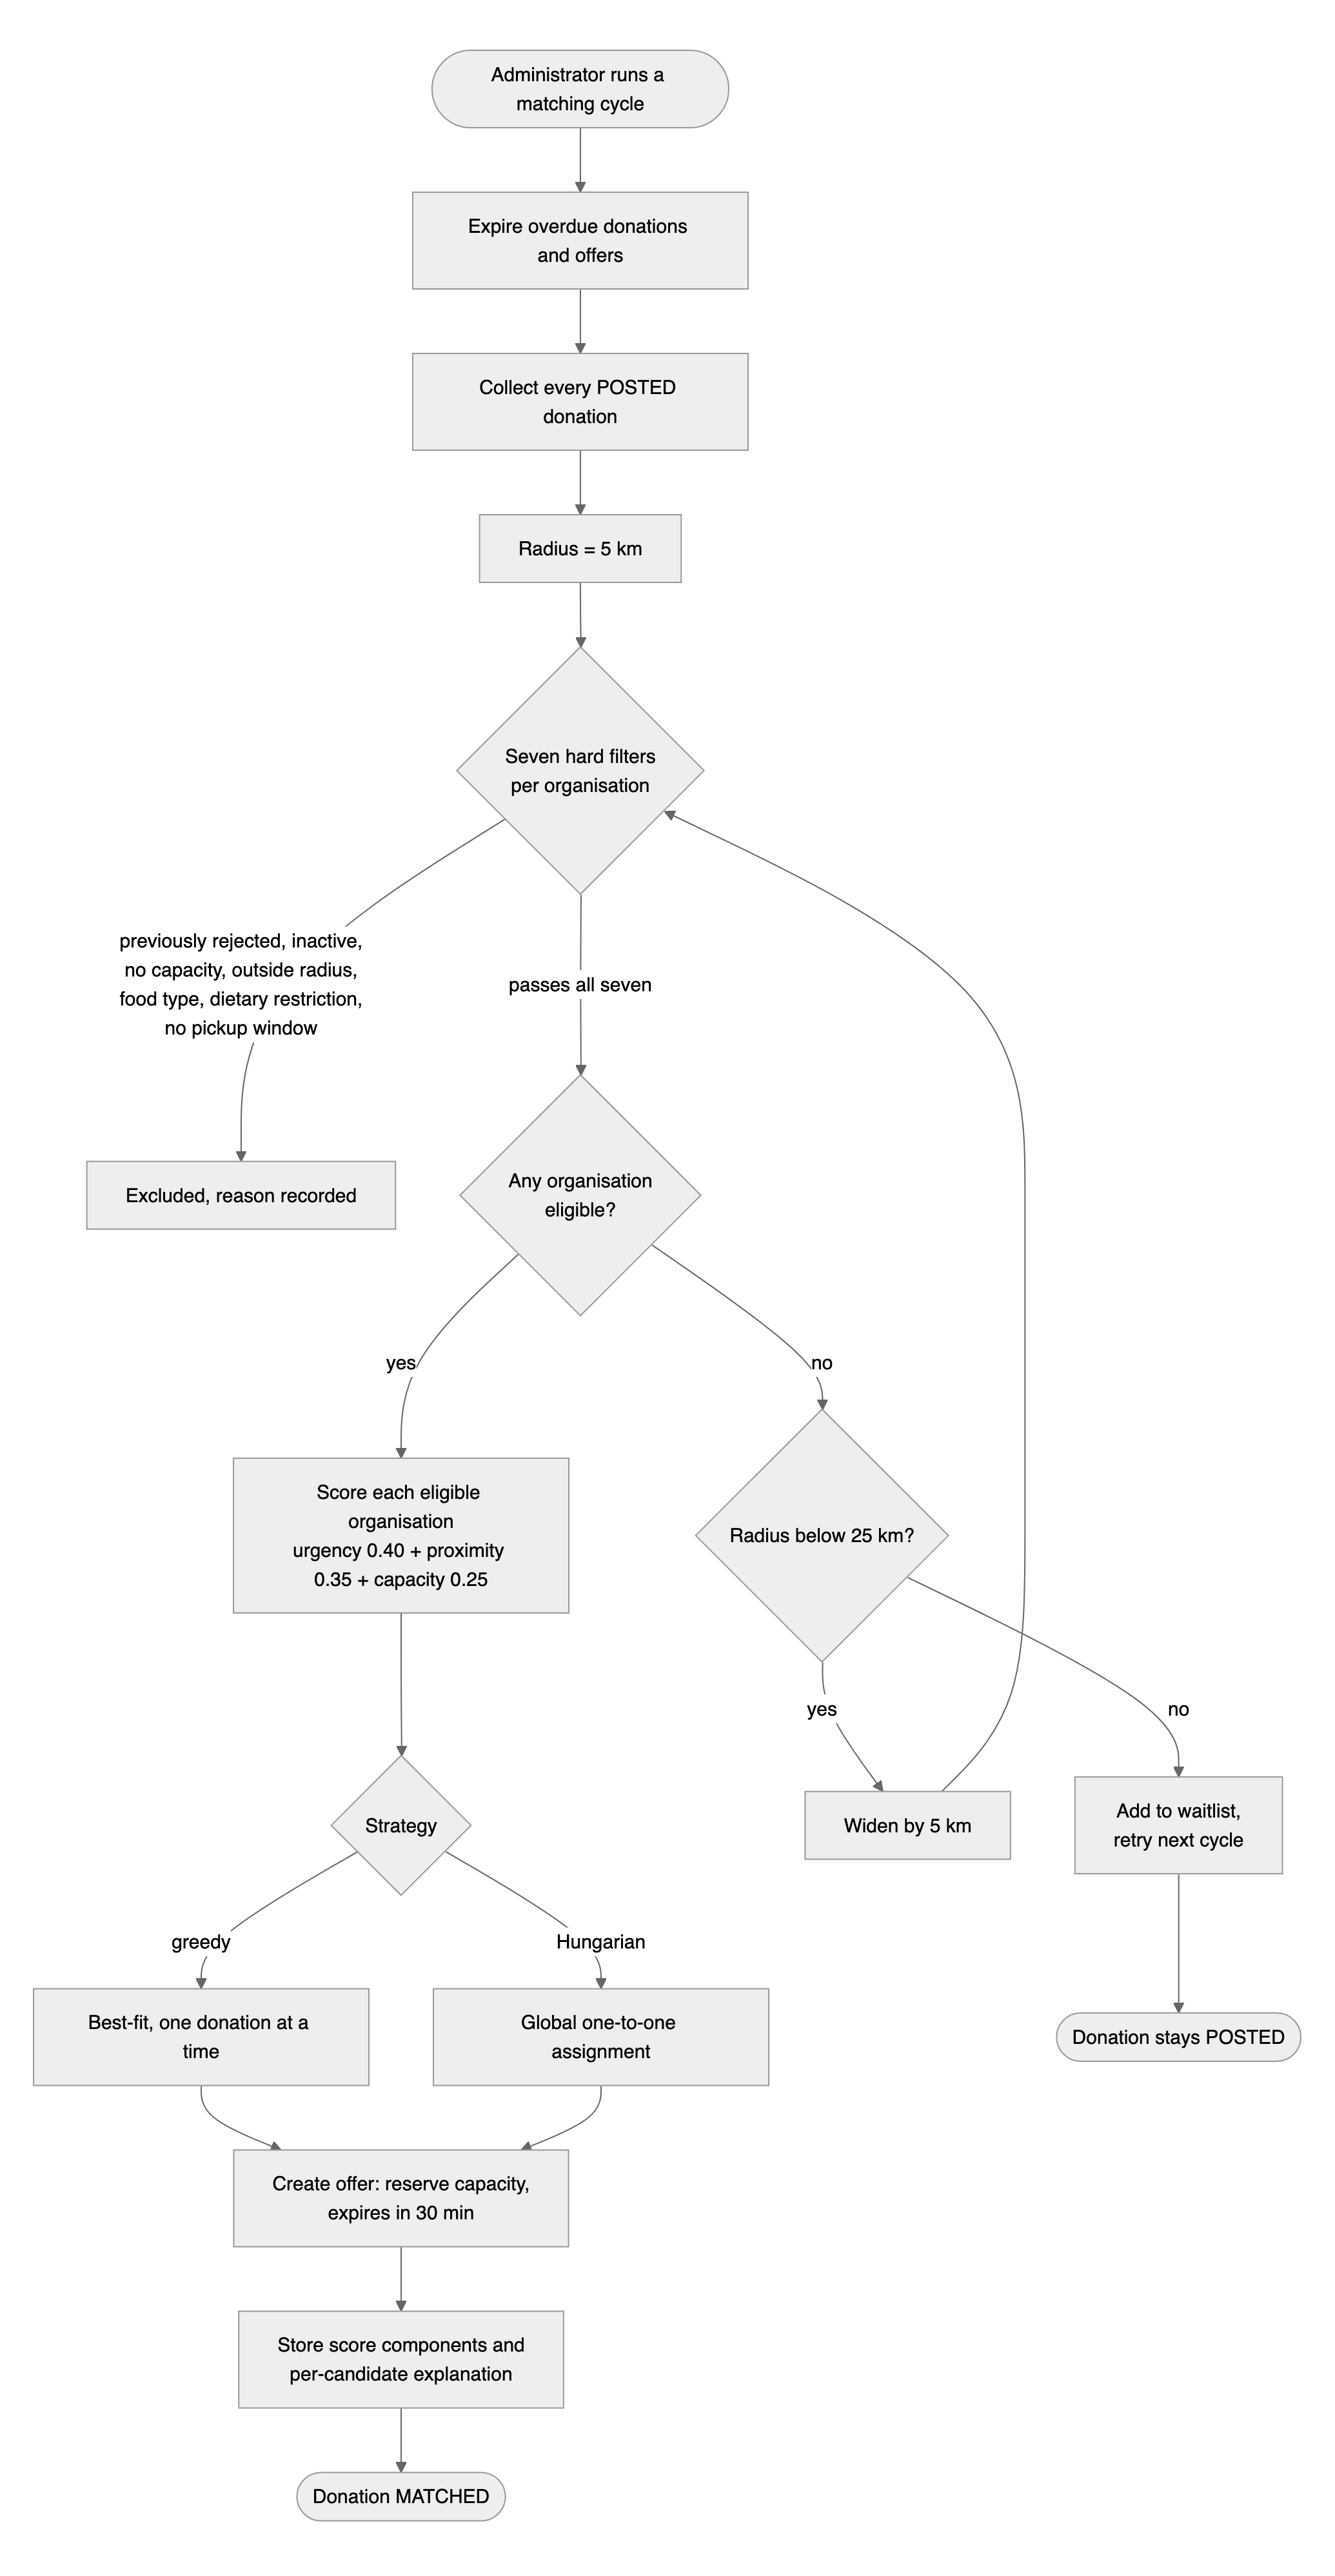
\includegraphics[height=0.82\textheight]{figures/activity.png}
\caption{Activity diagram of one matching cycle.}
\label{fig:activity}
\end{figure}

\paragraph{Sequence Diagram.}
Figure~\ref{fig:sequence} follows one donation from a typed address to a
completed pickup, through every service it touches. The cache lookup before the
call to Nominatim is what keeps the external provider out of the common path.

\begin{figure}[H]
\centering
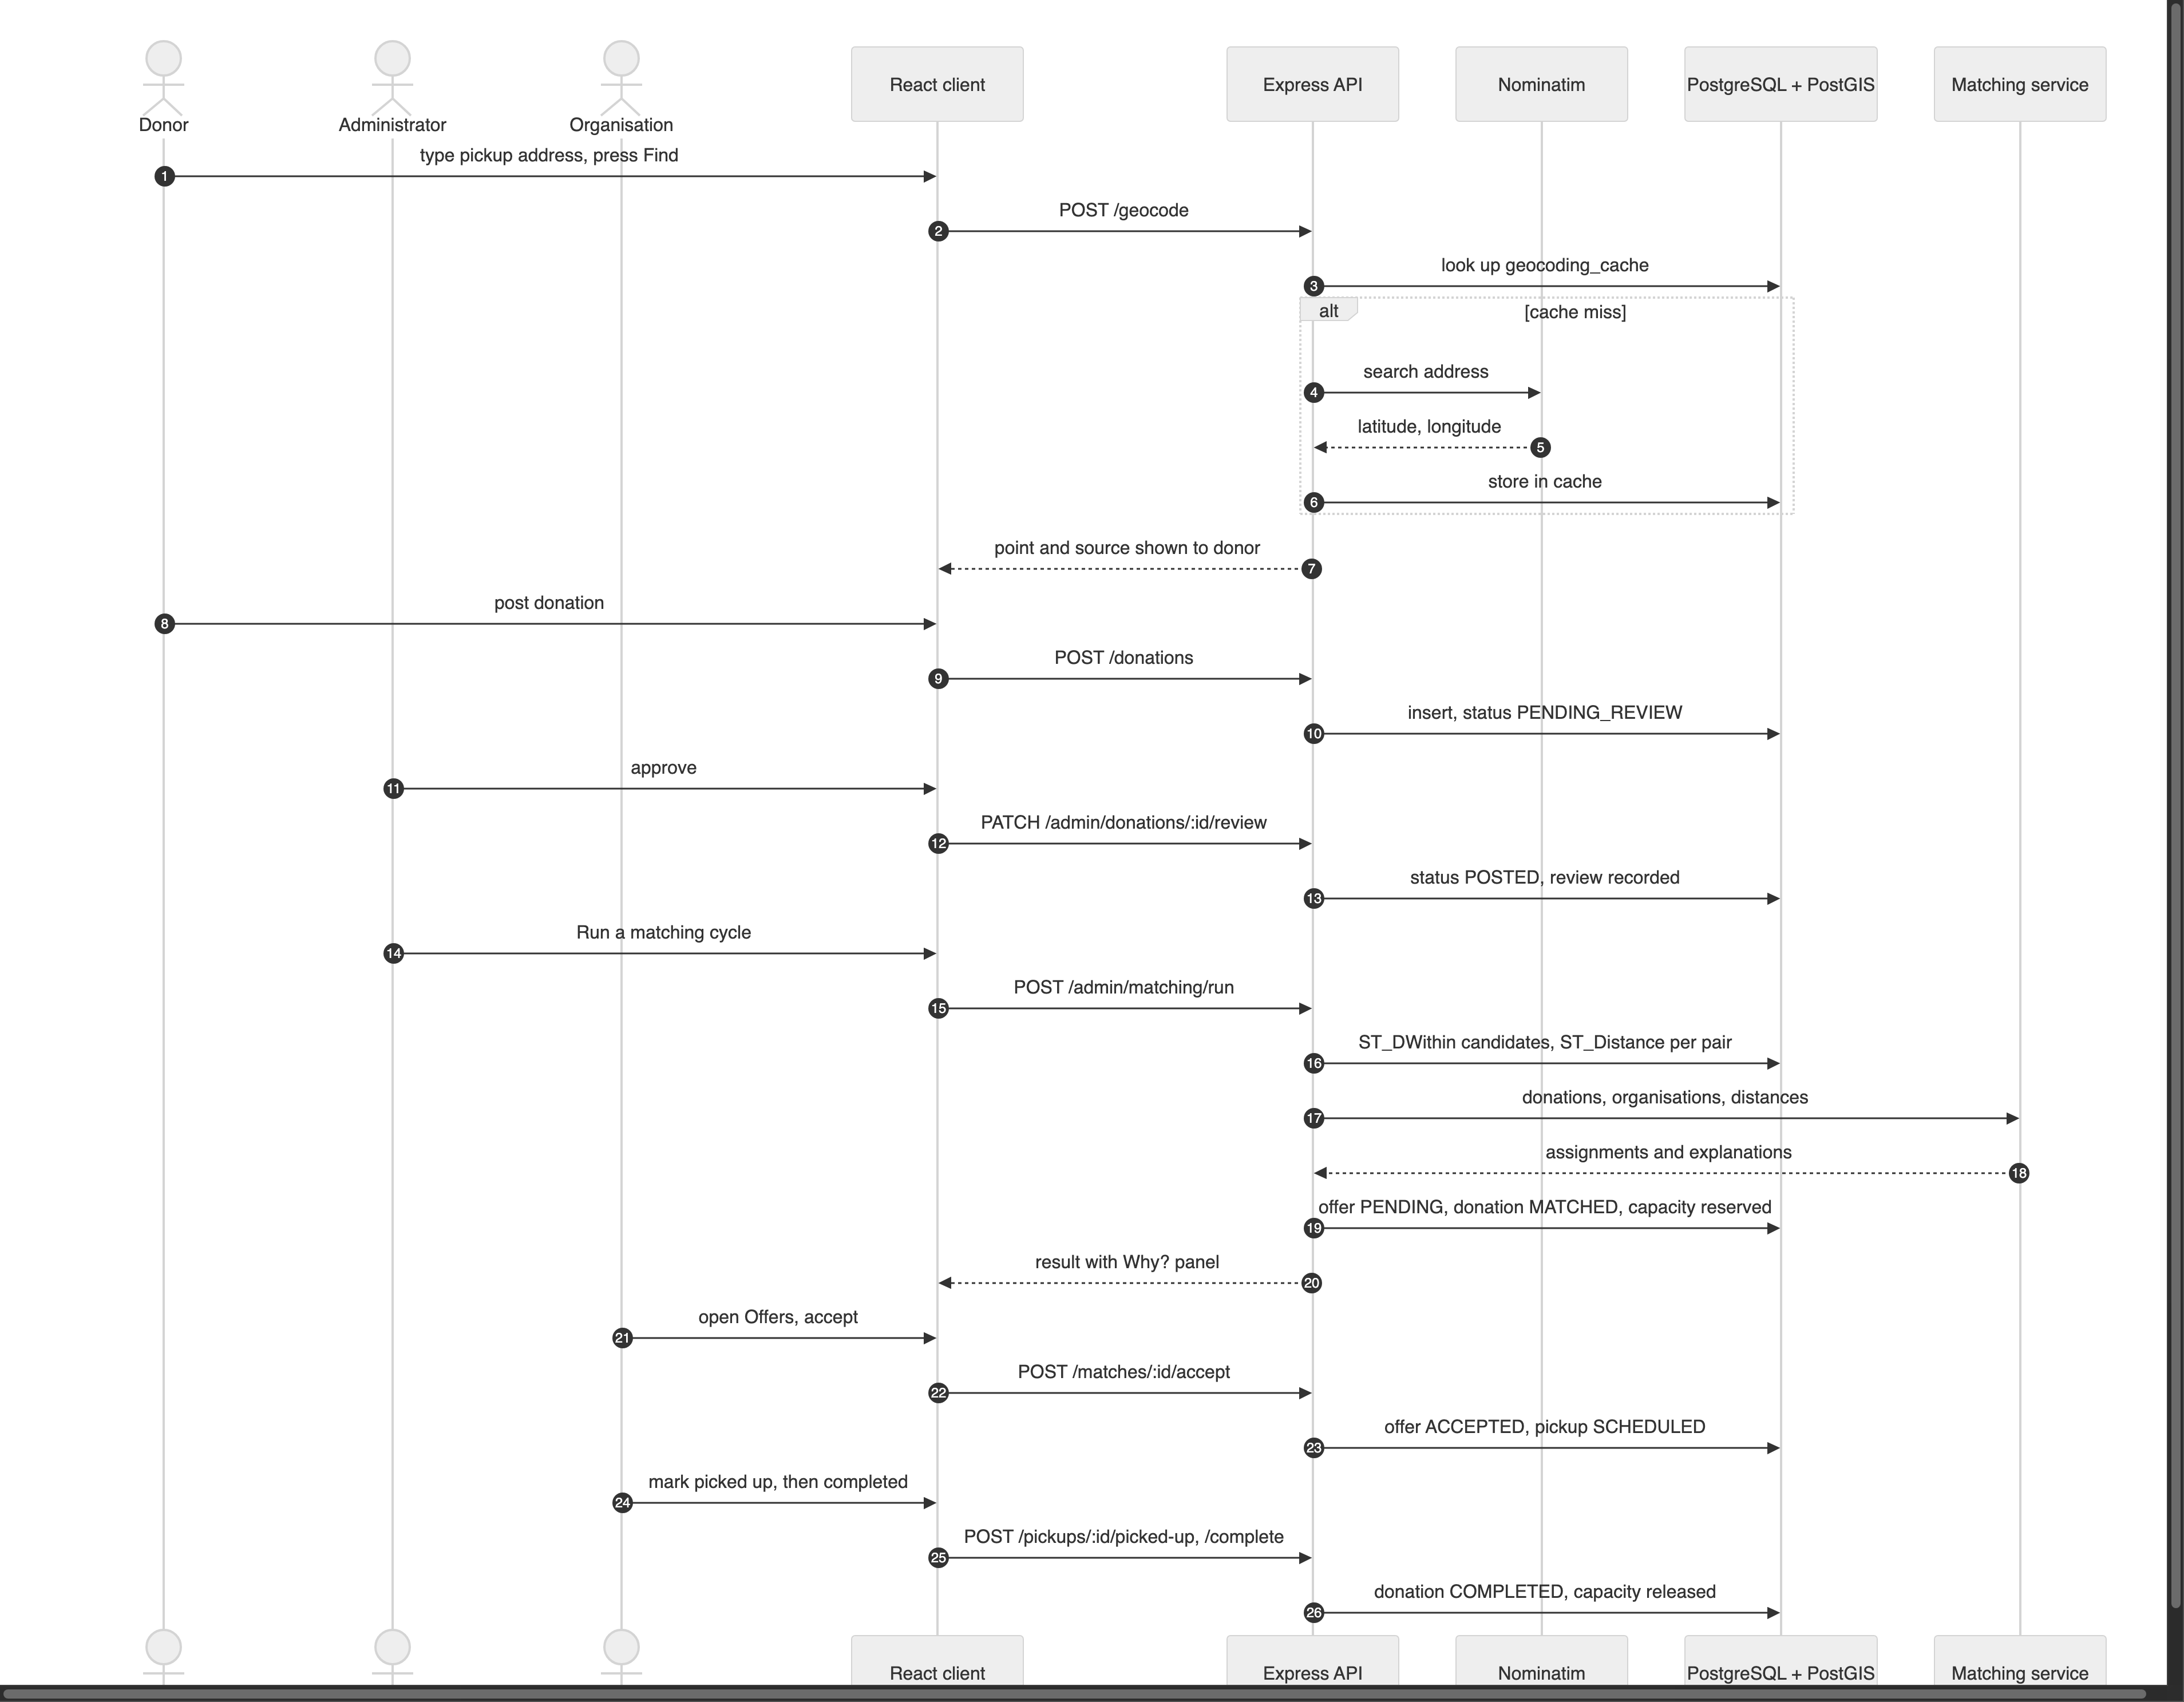
\includegraphics[width=\linewidth]{figures/sequence.png}
\caption{Sequence diagram: from a typed address to a completed pickup.}
\label{fig:sequence}
\end{figure}

\section{Implementation Details}

\subsection{Module 1: Accounts, Roles and Authentication}

Donors and recipient organisations register themselves; administrators cannot.
The registration endpoint accepts only the two self-service roles, so an
administrator account exists only if the operating team creates it. Passwords
are stored as bcrypt hashes and never returned. Every request after sign-in
carries a token from which the server derives the caller's role, and each route
states which roles may call it, so a donor reaching an administrator route is
refused with HTTP 403 rather than relying on the interface to hide the button.

\subsection{Module 2: Donation Submission and Geocoding}

A donor describes the food, its quantity in servings, how long it will remain
safe, and where it can be collected. The address is the part that needed most
care. Matching is spatial, so every donation must become a point, but asking a
canteen manager for latitude and longitude is unreasonable. The client therefore
sends the typed address to \code{POST /api/geocode}, which checks the database
cache first and only on a miss asks Nominatim, then shows the resolved point
before anything is submitted (Figure~\ref{fig:screens}a). An address that
silently resolved to the wrong town would quietly ruin every match that followed;
showing it first lets the donor catch that.

The endpoint is deliberately unauthenticated, because an organisation has to
locate its own address while it is still registering and has no token yet.
Because it reaches an external provider whose usage policy applies to the whole
application, it is rate-limited per caller instead.

\subsection{Module 3: Administrative Review}

No donation reaches an organisation without an administrator's approval. This
is the screening step for listing quality and food safety: the administrator
can approve, or reject with remarks, and every decision is stored with its
author and time. A second review of the same donation is refused, so a decision
cannot be silently overwritten.

\subsection{Module 4: The Matching Engine}

A cycle first applies seven hard filters to every organisation within the
maximum radius. An organisation is excluded if it has already declined this
donation, is inactive, lacks enough \emph{remaining} capacity, lies outside the
current search radius, does not accept the food type, has declared it as a
dietary restriction, or could not realistically collect it before the deadline.

The survivors are scored on three normalised components, with weights held as
configuration rather than written into the code:

\begin{table}[H]
\centering
\small
\begin{tabular}{@{}lcl@{}}
\toprule
\textbf{Component} & \textbf{Weight} & \textbf{What it rewards} \\
\midrule
Urgency   & 0.40 & donations closest to their deadline \\
Proximity & 0.35 & organisations closer to the pickup point \\
Capacity fit & 0.25 & a quantity that fits the remaining capacity well \\
\bottomrule
\end{tabular}
\caption{Scoring weights.}
\end{table}

Two allocation strategies are available per cycle. \emph{Greedy} assigns each
donation, most urgent first, to its best-scoring eligible organisation.
\emph{Hungarian} solves a global one-to-one assignment over all open donations at
once. If no organisation is eligible, the radius starts at 5\,km and widens in
5\,km steps to 25\,km; beyond that the donation is waitlisted and retried on
every later cycle. Each offer reserves the organisation's capacity for thirty
minutes, so the same capacity can never be promised to two donations.

Every cycle returns, for each donation, every organisation it weighed with its
distance and either its score or the reason it was excluded. The administrator
screen shows this under a \emph{Why?} button (Figure~\ref{fig:why}), which
turns the system's most important property --- that it can justify every
decision --- into something visible rather than claimed.

\subsection{Module 5: Offers, Pickup and Completion}

An organisation sees only offers made to it, each with the score components
that produced it. Accepting creates a scheduled pickup and discloses the two
parties' contact details, which are withheld until then. Declining returns the
donation to the pool and excludes that organisation from its immediate retry.
The collecting organisation then marks the food picked up and finally confirms
receipt, which completes the donation and releases its reserved capacity in a
single transaction. Once complete, both parties can rate from 1 to 5 how clearly
the status updates kept them informed; each sees only its own score.

\subsection{Module 6: Expiry, Audit Trail and Notifications}

A scheduler sweeps every sixty seconds without any administrator action,
expiring donations past their deadline and offers past their thirty-minute
window, and releasing the capacity they held. Every status change is written to
an audit table with its time and the user who caused it, which feeds the
timeline on each donation. The affected parties receive an in-app notification
at every transition.

\subsection{Module 7: Impact Reporting and Deployment}

The impact dashboard (Figure~\ref{fig:screens}b) reports meals redistributed,
median and mean time-to-match against the proposal's 20-minute target, rescue
rate, first-offer acceptance, the unmatched rate, food lost to expiry, waste
diverted, and mean donor-to-recipient distance for each allocation strategy.
Every figure is computed on the server from stored timestamps; the browser never
derives a metric, so the number on screen is the number quoted in this report.

The client is deployed on Vercel. The API, matching service and database run on
a team member's machine and are reached through a tunnel, so the live
deployment is available only while that machine is running.

\begin{figure}[H]
\centering
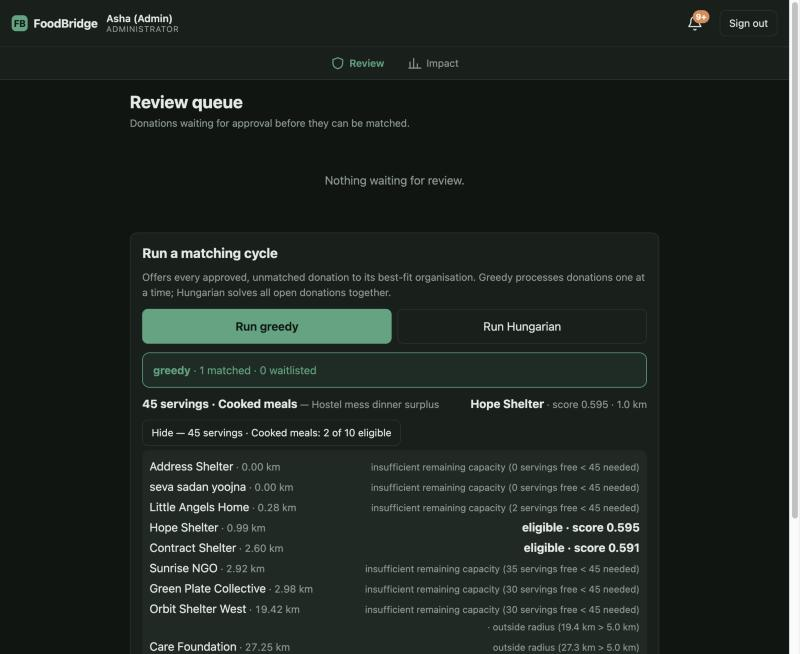
\includegraphics[width=0.94\linewidth]{figures/screen-why.jpg}
\caption{A matching cycle's \emph{Why?} panel. Every organisation the cycle
weighed is listed with its distance and either its score or the reason it was
excluded. Here the organisation 0.99\,km away narrowly outscored the one at
2.60\,km, while three closer organisations were excluded for lack of capacity.}
\label{fig:why}
\end{figure}

\begin{figure}[H]
\centering
\begin{subfigure}[t]{0.49\linewidth}
  \centering
  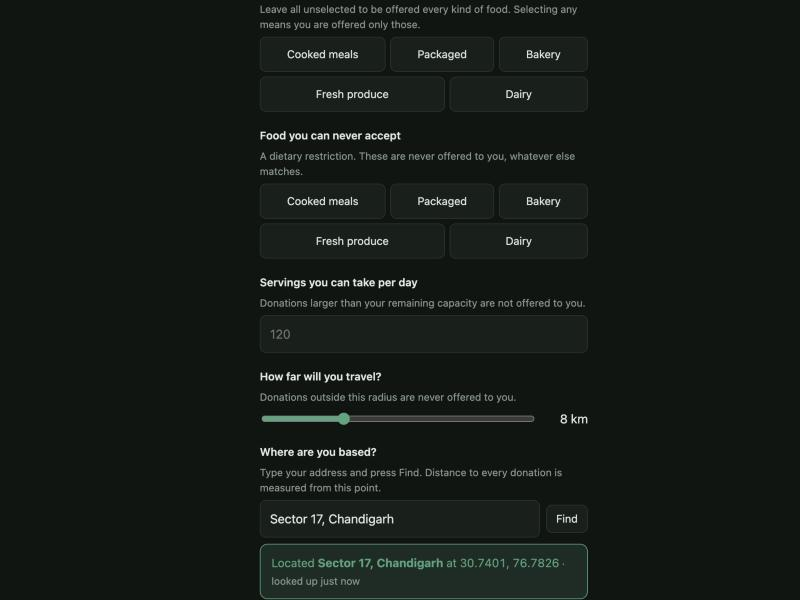
\includegraphics[width=\linewidth]{figures/screen-register.jpg}
  \caption{Registering by address. The resolved point is shown before
  submission.}
\end{subfigure}\hfill
\begin{subfigure}[t]{0.49\linewidth}
  \centering
  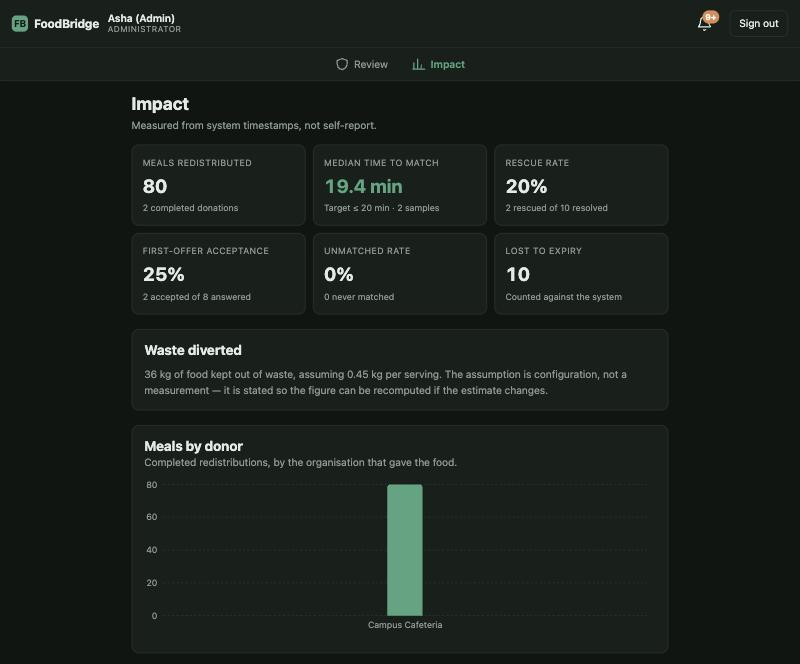
\includegraphics[width=\linewidth]{figures/screen-impact.jpg}
  \caption{Impact dashboard, computed on the server from stored timestamps.}
\end{subfigure}
\caption{Screens from the running application.}
\label{fig:screens}
\end{figure}

% ============================================================ Chapter 3
\chapter{Results and Evaluation}

\section{Testing Methodology}

Testing was organised around the places where the system can fail, at three
levels.

\paragraph{Unit and algorithm tests.} Thirty pytest cases exercise the matching
service in isolation: each hard filter, the scoring functions, greedy and
Hungarian allocation, and radius expansion.

\paragraph{API integration tests.} Eighty-four Vitest tests run the Express API
against a real PostgreSQL and PostGIS database rather than a mock, because
spatial queries and the state machine are exactly what a mock would hide.

\begin{table}[H]
\centering
\small
\begin{tabular}{@{}lr@{}}
\toprule
\textbf{Suite} & \textbf{Tests} \\
\midrule
State machines (every legal and illegal transition) & 16 \\
Backend completion: expiry, scheduler, audit trail & 11 \\
Integration refinements: ratings, metrics, refusals & 11 \\
Matching flow, end to end & 10 \\
Donation review & 10 \\
Geocoding and registration by address & 9 \\
Cycle explanations & 7 \\
Authentication and roles & 6 \\
Clarity rating on the donation detail & 4 \\
\midrule
\textbf{Total} & \textbf{84} \\
\bottomrule
\end{tabular}
\caption{Backend test suites.}
\end{table}

\paragraph{Contract tests.} A separate checker drives a running server through
every endpoint the React client depends on --- 32 checks covering status codes,
response shapes, the error envelope and role restrictions --- and exits non-zero
on any failure. It answers one question the other suites cannot: whether this
client can talk to this server without changes.

\paragraph{Continuous integration.} GitHub Actions runs the backend tests against
a PostGIS service container, the matcher tests, and a frontend lint and build on
every push. All three pass on the current \code{main}.

\paragraph{Checking the tests themselves.} A test that passes proves little unless
it would fail without the code it guards. For the cycle explanations, the
feature was removed deliberately and the suite re-run: five of its seven tests
failed, and all seven passed again once the feature was restored.

\section{Performance Metrics}

Latencies were measured with the API, matching service and database on one
machine. They show how long the backend itself takes, without the network delay
a user would add.

\begin{table}[H]
\centering
\small
\begin{tabular}{@{}lrr@{}}
\toprule
\textbf{Operation} & \textbf{Median (ms)} & \textbf{p95 (ms)} \\
\midrule
Sign in (bcrypt verification) & 52.0 & 52.7 \\
Donation detail, with full audit trail & 2.3 & 18.8 \\
Geocode, cache hit & 1.9 & 2.0 \\
Impact summary & 4.2 & 5.6 \\
Matching cycle: 10 donations, 100 candidate pairs & 107.3 & --- \\
\bottomrule
\end{tabular}
\caption{Measured latencies.}
\end{table}

Sign-in is the slowest common operation, and deliberately so: bcrypt is designed
to be expensive, which is what makes stolen hashes costly to attack. A cached
geocode takes under 2\,ms, whereas a fresh lookup is paced to Nominatim's
one-request-per-second policy --- the cache is what keeps that delay out of the
common path. A full matching cycle over a hundred donation--organisation pairs,
including the PostGIS distance computation and the round trip to the matcher,
completes in about a tenth of a second.

The spatial index is used rather than merely present: the query plan for a 5\,km
radius search is an index scan on the GiST index, not a sequential scan over
every organisation.

\section{Analysis}

\paragraph{From mid-semester to now.} Table~\ref{tab:progress} compares the
prototype presented at mid-semester with the current system.

\begin{table}[H]
\centering
\small
\begin{tabularx}{\linewidth}{@{}l>{\raggedright\arraybackslash}X>{\raggedright\arraybackslash}X@{}}
\toprule
\textbf{Area} & \textbf{Mid-semester} & \textbf{Now} \\
\midrule
Locations & Five preset places with fixed coordinates; the geocoding service
  existed but nothing could reach it & Any address, resolved and shown before
  submission; organisations can register by address \\
Dietary needs & Captured nowhere & A hard filter in matching, set at registration \\
Expiry & Only when an administrator ran a cycle & Unattended, every 60 seconds \\
Explanations & Stored, never shown & Visible for every candidate on the
  administrator screen \\
Audit trail & None & Every status change, with its time and actor \\
Evaluation metrics & No acceptance or distance data & Rescue rate, first-offer
  acceptance, distance per strategy \\
Clarity rating & Not built & Collected after completion \\
Tests & 42 API, 28 matcher, 23 contract & 84 API, 30 matcher, 32 contract \\
\bottomrule
\end{tabularx}
\caption{Progress since mid-semester.}
\label{tab:progress}
\end{table}

\paragraph{Three scenarios.} The system was demonstrated in three areas chosen so
that each shows a different property. At Thapar Institute, a 40-serving donation
went through every stage from posting to rating, and was offered to an
organisation 0.99\,km away. In Chandigarh, a 60-serving donation was offered to
the organisation at the pickup point while two others nearby were excluded for
two different reasons --- one did not accept cooked meals, and one had only 10
servings of capacity --- and organisations 34 to 58\,km away were excluded on
radius. In Manali, a donation with no organisation within 172\,km was waitlisted
rather than dropped, and was matched in the next cycle once a local organisation
registered.

\paragraph{Greedy against Hungarian.} The two strategies are better on different
measures, not one better overall. On one run, the Hungarian assignment placed food
at a mean of 1.27\,km against greedy's 3.65\,km, but made 3 offers against
greedy's 8. Because it solves a one-to-one assignment, an organisation receives
at most one donation per cycle; in a capacity-contention scenario greedy placed
two donations where Hungarian placed one. This comparison comes from whichever
cycles happened to run and is indicative, not a controlled experiment.

\paragraph{Where the defects were.} Almost every significant defect found during
development sat at a boundary between two parts that were each correct on their
own.
\begin{itemize}
  \item The registration form never sent an organisation's food preferences or
    dietary restrictions. Both fields existed in the schema, the repository, the
    API, the matcher client and the matcher's own model, and every test at every
    layer passed --- the one missing place was the form, the only place a user
    can enter a value.
  \item Donations were reaching no organisation at all because the form sent
    food types in one vocabulary and organisations stored them in another, and
    the matcher compares them exactly.
  \item The geocoding endpoint was first placed behind authentication, which made
    registration by address impossible, since a registering organisation has no
    token. No test caught it because every test already had one.
  \item One of four address shortcuts on the form, \emph{Model Town, Patiala},
    has no entry in OpenStreetMap, so pressing it failed. The geocoding tests did
    not catch it because they deliberately seed the cache to stay offline ---
    proving the cache works proves nothing about whether a particular address
    exists. It was replaced with one that resolves.
  \item The design diagrams carried over from the proposal had drifted from the
    code: they showed a pickup code that was never built and a donation state
    that does not exist. They were redrawn from the implementation for this
    report.
\end{itemize}

\paragraph{What the dashboard figures do and do not show.} The impact dashboard
currently reports a 20\% rescue rate and a median time-to-match of 19.4 minutes.
These come from development and demonstration use, where many donations were
created deliberately to test expiry and then left to lapse. They show that the
metrics are computed correctly from real timestamps; they are not evidence of how
the system would perform in real operation, which would need real donors.

% ============================================================ Chapter 4
\chapter{Conclusion}

\section{Summary of Work}

FoodBridge delivers the full redistribution workflow: registration by address,
donation posting, administrative approval, spatial matching with explicit and
configurable criteria, offers, pickup, completion and a post-completion rating.
It runs as three services over PostgreSQL and PostGIS, with the client deployed
publicly, and is covered by 84 API tests, 30 matcher tests and 32 contract
checks that run on every push.

\section{Key Findings}

\begin{enumerate}
  \item \textbf{Deciding eligibility before scoring changes the outcome.} Because
    an organisation that fails a hard constraint never competes, the nearest
    organisation is often not the one that receives the food, and the system can
    state exactly why.
  \item \textbf{The useful property of an allocation is that it can be
    explained.} Storing every candidate and its reason was cheap; showing it was
    what made the matching trustworthy to someone watching it.
  \item \textbf{Defects concentrate at boundaries.} Every serious defect above
    sat between two parts that each passed their own tests. Walking the interface
    as a user found them in minutes; no unit test could have.
  \item \textbf{No single allocation strategy is best.} The global assignment
    placed food closer; greedy placed more of it. The right choice depends on
    which outcome matters more.
\end{enumerate}

\section{Future Work and Recommendations}

\begin{enumerate}
  \item \textbf{Scheduled re-matching.} Expiry is already automatic, but matching
    still waits for an administrator. Running cycles on a timer is the change
    with the most direct effect on time-to-match.
  \item \textbf{Address precision checks.} The geocoder accepts any string it can
    resolve, including a whole state, and presents it with the same confidence as
    a street address. Nominatim already returns the precision of each result;
    rejecting anything coarser than a neighbourhood would stop a donation being
    posted to the middle of a region.
  \item \textbf{Organisation verification.} Legitimacy is currently screened per
    donation. Verifying organisations once, with registration documents, would
    move that burden off every listing.
  \item \textbf{E-mail and SMS notification.} Notifications are in-app only, which
    assumes the organisation is looking at the screen within the thirty-minute
    offer window.
  \item \textbf{A controlled strategy comparison.} Running both strategies over an
    identical set of donations would turn the indicative comparison above into a
    result.
\end{enumerate}

\section{Final Remarks}

The project set out to replace an informal, phone-and-message practice with a
workflow whose decisions are recorded, explainable and measurable. The system
now makes those decisions on stated criteria, shows its reasoning for every one,
and keeps food in the queue rather than losing it when nobody can take it. What
it cannot yet show is real-world impact, because that needs real donors and real
organisations using it over time --- and the measurements needed to judge that
are already in place.

\end{document}
